\documentclass[kulak]{kulakarticle}

\usepackage{amsmath}
\usepackage{amssymb}
\usepackage{amsfonts}
\usepackage{amsthm}
\usepackage{tcolorbox}
\usepackage{mathtools}
\usepackage{siunitx}
\usepackage{cancel}
\usepackage{mathtools}

\DeclareUnicodeCharacter{2212}{I~AM~HERE!!!!}

\let\epsilon\varepsilon

\newcommand{\R}{\mathbb{R}} % Real numbers
\newcommand{\C}{\mathbb{C}} % Complex numbers
\newcommand{\Q}{\mathbb{Q}}
\newcommand{\N}{\mathbb{N}}

\DeclareSIUnit\biti{bit_i}
\DeclareSIUnit\symbool{symbool}
\DeclareSIUnit\symbolen{symbolen}
\DeclareSIUnit\combinatie{combinatie}
\DeclareSIUnit\baud{baud}
\newcommand{\sam}{\text{sam}}

\DeclarePairedDelimiter\abs{\lvert}{\rvert}
\usepackage{array}
\usepackage{multirow}

\sisetup{output-decimal-marker={.}}
\sisetup{per-mode=symbol}
\sisetup{per-symbol=/}
\sisetup{group-digits=integer}

\newcommand{\rood[1]}{\color{red}#1\color{black}}

\usepackage[dutch]{babel}
\usepackage{hyperref}

%\setlength{\parindent}{0pt}
% d voor dx
\newcommand*\diff{\mathop{}\!\mathrm{d}}

\usepackage{parskip}

\title{Examen Informatieoverdracht en -verwerking}
\author{Vincent Van Schependom}
\date{9 januari 2025}
\address{
	\textbf{Informatieoverdracht en -verwerking}\\
	Prof. Lieven De Lathauwer \& Ben Hermans}

\begin{document}

	\maketitle

	\section*{Vraag 1}

	Een koning maakt een random walk op een 3x3 schaakbord met posities 1 tot en met 9. We kunnen dit modelleren door de hoeken te benoemen met \(H\), de posities aan de zijden met \(R\), en het midden met \(C\).

	\renewcommand{\arraystretch}{1.5}
	\begin{table}[h!]
		\centering
		\begin{tabular}{|c|c|c|}
			\hline
			1 & 2 & 3 \\
			\hline
			4 & 5 & 6 \\
			\hline
			7 & 8 & 9 \\
			\hline
		\end{tabular}
		\hspace{2cm}
		\begin{tabular}{|c|c|c|}
			\hline
			\(H\) & \(R\) & \(H\) \\
			\hline
			\(R\) & \(C\) & \(R\) \\
			\hline
			\(H\) & \(R\) & \(H\) \\
			\hline
		\end{tabular}
	\end{table}

	\begin{enumerate}
		\item Bereken de gemiddelde hoeveelheid informatie voor een voorstelling \(\{R,H,C\}\) na heel veel stappen.
		\item We duiden nu elke positie aan m.b.v. diens getal. Wat zijn de kansen voor een voorstelling \(\{1,2,...,9\}\)? Bereken ook hiervoor de gemiddelde hoeveelheid informatie.
		\item Als we de positie van de koning doorsturen door eerst de rij en vervolgens de kolom door te geven, bestaat er dan een afhankelijkheid tussen de rijen en kolommen? Leg uit.
		\item Maak een Huffman-codering voor een voorstelling \(\{1,2,...,9\}\). Bereken de gemiddelde codewoordlengte, de efficiëntie en de compressieverhouding van je codering.
	\end{enumerate}

	\underline{Oplossing}:

	\begin{enumerate}

		\item We kunnen dit probleem modelleren aan de hand van een Markov keten. Voor de overgangskansen vinden we dat \begin{align*}
			\mathbf{C} = \begin{bmatrix}
				P(H\, | \,H) & P(H\, | \,C) & P(H\, | \,R) \\
				P(C\, | \,H) & P(C\, | \,C) & P(C\, | \,R) \\
				P(R\, | \,H) & P(R\, | \,C) & P(R\, | \,R)
			\end{bmatrix} = \begin{bmatrix}
				0 			& \frac{1}{2} 	& \frac{2}{5} \\
				\frac{1}{3} & 0 			& \frac{1}{5} \\
				\frac{2}{3} & \frac{1}{2}	& \frac{2}{5}
			\end{bmatrix}
		\end{align*}We bereiken een steady state wanneer \[\mathbf{p}_k = \mathbf{p}_{k+1} = \mathbf{C}\mathbf{p}_k = \mathbf{p} \quad \Longleftrightarrow \quad (\mathbf{C}-\mathbb{I}_3)\mathbf{p}=0.\] Omdat dit stelsel oneindig veel oplossingen heeft, voegen we de voorwaarde \(\sum_{i=1}^{3} p(x_i) = 1\) toe, waarbij \(x_1=H, x_2=C\) en \(x_3=R\). We stoppen dit in de PlySmlt2 simultaneous equation solver van onze trusty TI-84 en er bolt een unieke oplossing uit. \begin{align*}
			\begin{bmatrix}
				\mathbf{C} - \mathbb{I}_3 \\
				1
			\end{bmatrix}\mathbf{p} = \begin{bmatrix}
			0 \\
			1
			\end{bmatrix} \quad \Longleftrightarrow \quad \mathbf{p} = \begin{bmatrix}
			P(H)\\
			P(C)\\
			P(R)
			\end{bmatrix} = \begin{bmatrix}
			\frac{3}{10}\\
			\frac{1}{5}\\
			\frac{1}{2}
			\end{bmatrix}
		\end{align*}
		We kunnen nu de gemiddelde hoeveelheid informatie berekenen:
		\begin{align*}
			H(\{R,H,C\}) = - \sum_{i=1}^{3} p(x_i) \log p(x_i) = \SI{1.48}{\biti\per\symbool}
		\end{align*}

		\item Omdat er 4 \(H\)-steentjes zijn, 4 \(R\)-steentjes zijn en 1 \(C\)-steentje is, geldt dat \begin{align*}
			P(1) = P(3) = P(7) = P(9) &= \frac{P(H)}{4} &=&\, \frac{3}{40}\\
			P(2) = P(4) = P(6) = P(8) &= \frac{P(R)}{4} &=&\, \frac{1}{8} \\
			P(5) &=P(C) &=&\, \frac{1}{5}.
		\end{align*} Voor de gemiddelde hoeveelheid informatie vinden we nu dat \begin{align*}
		H(\{1,2,...,9\}) &= - \sum_{i=1}^{9} P(i) \log P(i)\\
						&= - \left[ 4 \cdot \frac{3}{40} \log\left(\frac{3}{40}\right) + 4 \cdot \frac{1}{8} \log\left(\frac{1}{8}\right) + \frac{1}{5} \log\left(\frac{1}{5}\right) \right] \\
						&= \SI{3.085}{\biti\per\symbool}
		\end{align*}

		\item We controleren of \(P(K_i, R_j) = P(K_i) \cdot P(R_j)\). Hiervoor berekenen we bijvoorbeeld de kolom- en rijkans voor \(K_2\) en \(R_2\): \begin{align*}
			P(K_2) &= P(2) + P(3) + P(8)\\
					&= \frac{1}{8} + \frac{1}{5} + \frac{1}{8} = \frac{9}{20}\\
					& = P(4) + P(3) + P(6) = P(R_2)
		\end{align*} Omdat nu geldt dat \begin{align*}
		P(R_2,K_2) = P(C) = \frac{1}{5} \neq P(R_2) \cdot P(K_2) = \left(\frac{9}{20}\right)^2,
		\end{align*} zijn de kansen duidelijk niet onafhankelijk.

		\item De Huffman-code heeft een gemiddelde codewoordlengte van \(L = 3.15 \, \frac{\text{symbolen uit \(B\)}}{\text{codewoord}}\). De efficiëntie bedraagt dus \[\epsilon = \frac{H(\{1,2,...,9\})}{L \cdot \log_2 2} = 0.98,\] en de compressiefactor is gelijk aan \[\frac{\lceil \log_2 9 \rceil}{3.15}=1.27.\]

	\end{enumerate}

	\section*{Vraag 2}

	Gegeven twee figuren met daarop het frequentiespectrum van twee filters; de linkerfiguur is een gewone plot en de rechterfiguur is een semilog plot. De ene filter is in het blauw getekend, de andere in het rood. Er geldt dat \(M=51\) en \(f_\text{sam}=\SI{100}{\mega\hertz}\). De cut-off frequentie voor de blauwe figuur is 1. De stopfrequentie van de blauwe filter is aangeduid op de rechterfiguur.

	\begin{enumerate}
		\item Welke windows worden hier gebruikt? Leg uit.
		\item Wat is de vertraging?
		\item Bepaal de doorlaatfrequentie, stopfrequentie en cut-off frequentie van de blauwe filter in Hertz.
		\item Bereken de breedte van de transitieband van de blauwe filter. Komt die overeen met de uitdrukking het eerder bepaalde window?
		\item Hoe zou een filter met een Hann window eruit zien? Teken deze filter op beide figuren en motiveer je schets.
	\end{enumerate}

	\underline{Oplossing}:

	\begin{enumerate}
		\item De filter in het blauw is het rechthoekig window: \begin{itemize}
			\item Meer rimpelingen
			\item Kleinere transitieband
			\item \(\delta_s = \SI{21}{\decibel}\) (figuur)
		\end{itemize}

		De filter in het rood is het Blackman window: \begin{itemize}
			\item Minder rimpelingen
			\item Grotere transitieband
			\item \(\delta_s = \SI{75}{\decibel}\) (figuur)
		\end{itemize}

		\item De vertraging is gelijk aan \begin{align*}
			(M-1) \cdot T_\text{sam} = \frac{(M-1)}{f_\text{sam}} = \frac{50}{100 \cdot 10^{6}} = \SI{50}{\micro\second}.
		\end{align*}

		\item Voor het rechthoekig window geldt voor de breedte van de transitieband gelijk is aan \(6/M\). Omdat \(\omega_s = 1.0588\) gegeven is op de figuur, kunnen we afleiden dat \begin{align*}
			\omega_s - \omega_p = \frac{6}{51} \quad \Longrightarrow \quad \omega_p  = \omega_s - \frac{6}{51} = (1.0588-0.11765) \,\SI{}{\radian} = 0.9412 \,\SI{}{\radian}.
		\end{align*} Omdat genormaliseerde frequenties gedefinieerd zijn als \(\omega_x = \frac{2\pi \cdot f_x}{f_\text{sam}}\), geldt dat \(f_x = \frac{\omega_x \cdot f_\text{sam}}{2 \pi}\): \begin{align*}
			f_p &= \frac{\omega_p \cdot f_\text{sam}}{2 \pi} = \frac{0.9412 \cdot 100 \cdot 10^6}{2 \pi} &= \SI{14.98}{\mega\hertz}\\
			f_c &= \frac{\omega_c \cdot f_\text{sam}}{2 \pi} = \frac{1 \cdot 100 \cdot 10^6}{2 \pi} &= \SI{15.92}{\mega\hertz}\\
			f_s &= \frac{\omega_s \cdot f_\text{sam}}{2 \pi} = \frac{1.0588 \cdot 100 \cdot 10^6}{2 \pi} &= \SI{16.85}{\mega\hertz}
		\end{align*}
	\end{enumerate}

	\section*{Vraag 3}

	Wanneer is de performantie van een \((n,k)\)-blokcode het hoogst? Hiermee bedoelen we: wanneer is het foutdetectievermogen maximaal? We beperken ons tot \(k=3\).

	\begin{enumerate}
		\item Geef de (\(4,3)\)-blokcode met de beste performantie en bepaal het foutdetecterend vermogen.
		\item Bepaal alle codewoorden van de zonet bepaalde blokcode en geef ook het foutcorrectievermogen.
		\item Bepaal de efficiëntie. Als je een extra kolom toevoegt, wat gebeurt er dan met de efficiëntie en de performantie van je blokcode?
	\end{enumerate}

	\underline{Oplossing}:

	\begin{enumerate}
		\item \renewcommand{\arraystretch}{1}
		Voor de generatormatrix \(\mathbf{G}\) vinden we dat \begin{align*}
			\mathbf{G} = \left[\begin{array}{c|c}
				\mathbb{I}_3 & \mathbf{P}
			\end{array}\right] = \left[\begin{array}{ccc|c}
				1 & 0 & 0 & a \\
				0 & 1 & 0 & b \\
				0 & 0 & 1 & c
			\end{array}\right]
		\end{align*}
		De blokcode is \textit{systematisch}, i.e. de eerste \(k=3\) symbolen van een codevector \(\mathbf{C}\) zijn gelijk aan de bronvector \(\mathbf{U}\). Daarnaast is de blokcode \textit{lineair}: de laatste \((k-n)=1\) symbolen van een codevector zijn een lineaire combinatie van rijen in de matrix \(\mathbf{P}\), modulo 2. De codevectoren zijn dus van de vorm \begin{align*}
			\begin{bmatrix}
				c_1 & c_2 & c_3 & c_4
			\end{bmatrix} = \begin{bmatrix}
				u_1 & u_2 & u_3
			\end{bmatrix} \cdot \mathbf{G} = \left[\begin{array}{ccc|c}
				u_1 & u_2 & u_3 & (u_1 a + u_2 b + u_3 c) \mod 2
			\end{array}\right].
		\end{align*}
		Om het foutdetecterend vermogen \(e=d_{\min} - 1\) zo klein mogelijk te maken, moeten we \(d_{\min}\) minimaliseren. Hierbij is \(d_{\min}\) de kleinste Hamming-afstand. Omdat de nulvector een codewoord is, is de kleinste Hamming-afstand gewoonweg het kleinste gewicht (i.e. het aantal eentjes) van de van nul verschillende codewoorden. Het aantal eentjes is minimaal voor een bronvector met slechts één enkele 1, dus voor \(\mathbf{U} = \begin{bmatrix}
			1 & 0 & 0
		\end{bmatrix}, \begin{bmatrix}
		0 & 1 & 0
		\end{bmatrix}\) of \(\begin{bmatrix}
		0 & 0 & 1
		\end{bmatrix}\). In dat geval is het laatste element van de overeenkomstige codevector \(\mathbf{C}\) gelijk aan \(a,b\) of \(c\). Opdat het gewicht van alle 3 de codevectoren, die overeenkomen met de eerder vermelde bronvectoren, 2 zou zijn, moet gelden dat \(a=b=c=1\).

		We hebben net de parameters \(a,b\) en \(c\) gelijkgesteld aan 1 om een minimaal gewicht van \(d_{\min}=1\) te bekomen. Hieruit volgt direct dat het foutdetecterend vermogen gelijk is aan \(e=2-1=1\).

		\item De codevectoren kunnen op een snelle manier berekend worden vanwege de systematische \& lineaire aard van de blokcode, zoals hierboven al werd aangehaald. We vinden: \begin{align*}
			\begin{bmatrix} 0 & 0 & 0 \end{bmatrix} & \rightarrow \begin{bmatrix} 0 & 0 & 0 & 0 \end{bmatrix} \\
			\begin{bmatrix} 0 & 0 & 1 \end{bmatrix} & \rightarrow \begin{bmatrix} 0 & 0 & 1 & 1 \end{bmatrix} \\
			\begin{bmatrix} 0 & 1 & 0 \end{bmatrix} & \rightarrow \begin{bmatrix} 0 & 1 & 0 & 1 \end{bmatrix} \\
			\begin{bmatrix} 1 & 0 & 0 \end{bmatrix} & \rightarrow \begin{bmatrix} 1 & 0 & 0 & 1 \end{bmatrix} \\
			\begin{bmatrix} 0 & 1 & 1 \end{bmatrix} & \rightarrow \begin{bmatrix} 0 & 1 & 1 & 0 \end{bmatrix} \\
			\begin{bmatrix} 1 & 1 & 0 \end{bmatrix} & \rightarrow \begin{bmatrix} 1 & 1 & 0 & 0 \end{bmatrix} \\
			\begin{bmatrix} 1 & 0 & 1 \end{bmatrix} & \rightarrow \begin{bmatrix} 1 & 0 & 1 & 0 \end{bmatrix} \\
			\begin{bmatrix} 1 & 1 & 1 \end{bmatrix} & \rightarrow \begin{bmatrix} 1 & 1 & 1 & 1 \end{bmatrix}
		\end{align*}
		We zien dus inderdaad dat voor \(a=b=c=1\) geldt dat \(d_{\min}=2\). Het foutcorrigerend vermogen is gelijk aan \begin{align*}
			t = \left\lfloor \frac{d_{\min}-1}{2} \right\rfloor = \left\lfloor \frac{1}{2} \right\rfloor = 0.
		\end{align*}

		\item De efficiëntie bedraagt \(\epsilon = k/n = 75\%\). Als we een extra kolom toevoegen, vermindert de efficiëntie (\(\epsilon' = k/n' = 60\%\)), maar zal de performantie van de blokcode niet veranderen. De minimale Hamming-afstand \(d_{\min}'\) blijft gelijk aan 2.
	\end{enumerate}

	\section*{Vraag 4}

	Een signaal wordt verstuurd in basisband aan een transmissiedebiet van \SI{60}{\kilo\bit\per\second}. Hiervoor worden \(M\) verschillende golfvormen gebruikt met factor \(\alpha = 0.75\). Verder geldt dat \(E_b/N_0=100\). We willen een foutkans die minder dan \(10^{-6}\) bedraagt.

	\begin{enumerate}
		\item Hoeveel golfvormen kunnen we maximaal versturen?
		\item Wat is de bandbreedte van dit signaal?
		\item We passen FDM toe van 100 tot \SI{180}{\kilo\hertz} met enkel-zijband modulatie, waarbij enkel de hoogste zijband wordt behouden. Hoeveel signalen kunnen we maximaal multiplexen? Stel dat we maximale spreiding willen -- ook bij \SI{100}{\kilo\hertz}, maar niet bij \SI{180}{\kilo\hertz}. Bepaal dan de draaggolffrequenties en teken het spectrum.
	\end{enumerate}

	\newpage
	\underline{Oplossing}:

	\begin{enumerate}
		\item	We voldoen aan de eis die wordt opgelegd voor de foutkans wanneer \begin{align*}
			P_g \leq 10^{-6} & \Longleftrightarrow \frac{2(M-1)}{M} Q \left( \sqrt{\frac{6 \log_2 M}{M^2 - 1} \cdot \frac{E_b}{N_0}} \right) \leq 10^{-6} \\
			& \Longleftarrow 2 Q \left( \sqrt{\frac{6 \log_2 M}{M^2 - 1} \cdot 100} \right) \leq 10^{-6} && \frac{2(M-1)}{M} < 2 \\
			& \Longleftrightarrow Q \left( \sqrt{\frac{600 \log_2 M}{M^2 - 1}} \right) \leq 5 \cdot 10^{-7} \\
			& \Longleftrightarrow \sqrt{\frac{600 \log_2 M}{M^2 - 1}} \geq 4.8  \\
			& \Longleftrightarrow \frac{\log_2 M}{M^2 - 1} \geq \frac{4.8^2}{600} = 0.0384 \\
			& \Longleftrightarrow M \leq 9
		\end{align*}

		We kiezen \(M=8\) zodat het een macht van 2 is: \(M=2^3 = 2^{n_s} \rightarrow n_s=3\).

		\item In basisband geldt dat \(B = (1 + \alpha)f_m\). De maximale frequentie is niet gegeven, maar kunnen we als volgt berekenen: \begin{align*}
			\left\{ \begin{array}{l}
				T_s = \dfrac{1}{2f_m} = \dfrac{1}{r_s} \\
				r_b = r_s \cdot n_s
			\end{array} \right. \quad \Longleftrightarrow \quad \left\{ \begin{array}{l}
			f_m = r_s/2 \\
			r_s = r_b/n_s
			\end{array} \right. \quad \Longleftrightarrow \quad f_m = \frac{r_b}{2n_s}
		\end{align*}
		We vinden dus dat \begin{align*}
			B = (1+\alpha)\cdot\frac{r_b}{2n_s} = (1+0.75)\cdot\frac{60 \cdot 10^3}{2 \cdot 3} \quad \Longrightarrow \quad B = \SI{17500}{\hertz} =  \SI{17.5}{\kilo\hertz}
		\end{align*}

		\item We hebben \SI{80}{\kilo\hertz} beschikbare bandbreedte om \(X\) signalen tussen te moduleren. Aangezien we Single Sideband modulatie doen (waarbij enkel de hoogste zijband behouden wordt), blijft de bandbreedte beperkt tot \SI{17.5}{\kilo\hertz} -- ook al zitten we nu in doorlaatband en niet meer in basisband. We vinden dat we \begin{align*}
			X = \left\lfloor \frac{80 \cdot 10^3}{17.5 \cdot 10^3} \right\rfloor = 4
		\end{align*} signalen kunnen multiplexen in doorlaatband. De overige \((80 - 4 \cdot 17.5) \, \SI{}{\kilo\hertz}\) delen we door 4, aangezien er vóór elke \textit{raised cosine} in het frequentiespectrum spreiding vereist is. Zo vinden we dat de spaties \SI{2.5}{\kilo\hertz} breed zijn.

		We berekenen de draaggolffrequenties: \begin{align*}
			f_{c_1} &= (100 + 2.5) \, \SI{}{\kilo\hertz} &= \SI{102.5}{\kilo\hertz} \\
			f_{c_2} &= f_{c_1} + (17.5 + 2.5) \, \SI{}{\kilo\hertz} &= \SI{122.5}{\kilo\hertz} \\
			f_{c_3} &= f_{c_2} + \SI{20}{\kilo\hertz} &= \SI{142.5}{\kilo\hertz} \\
			f_{c_4} &= f_{c_3} + \SI{20}{\kilo\hertz} &= \SI{162.5}{\kilo\hertz}
		\end{align*}
	\end{enumerate}

	\newpage
	\section*{Vraag 5}

	We ontwerpen een (kinder)slot met 3 cijfers. De invoer voor het slot zijn combinaties \(A_1 A_0\), die een binaire voorstelling zijn van de cijfers die werden gegeven. Bijvoorbeeld: \(01\) wil zeggen dat het cijfer 1 werd ingevoerd; \(11\) wil zeggen dat het cijfer 3 werd ingevoerd. De uitvoer van het slot is \(Y\) en is gelijk aan 0 wanneer een verkeerde combinatie werd ingevoerd en 1 wanneer de juiste combinatie -- namelijk 3, gevolgd door 0, gevolgd door 2 -- werd ingevuld. Wanneer een fout cijfer wordt gegeven, verwerpt het slot de volledige sequentie niet, maar blijft het in dezelfde toestand. Wanneer de correcte combinatie werd ingevuld, moet het slot automatisch terug naar de begintoestand gaan in de volgende klokcyclus.

	\begin{enumerate}
		\item Teken een Moore toestandsdiagram van dit slot.
		\item Codeer de toestanden aan de hand van straight-forward codering en Gray codering. Wat zijn de voordelen van elke codering? Tip: wat stelt de straight-forward codering van een toestand voor?
		\item Stel de waarheidstabel op voor de ingang, huidige toestand, volgende toestand en de output.
		\item Bepaal de SOP uitdrukkingen voor de volgende toestand en de output.
		\item Stel Karnaugh kaarten op voor de volgende toestand en de output. Bepaal minimale uitdrukkingen in Booleaanse logica met AND, OR en NOT.
		\item Teken de schakeling op een overzichtelijke manier op poortniveau.
		\item Voer in een andere kleur (of in het potlood) technologiemapping (CMOS) uit.
	\end{enumerate}

	\underline{Oplossing}
	\begin{enumerate}
		\item Toestandsdiagram:
		\begin{figure}[h!]
			\centering
			
		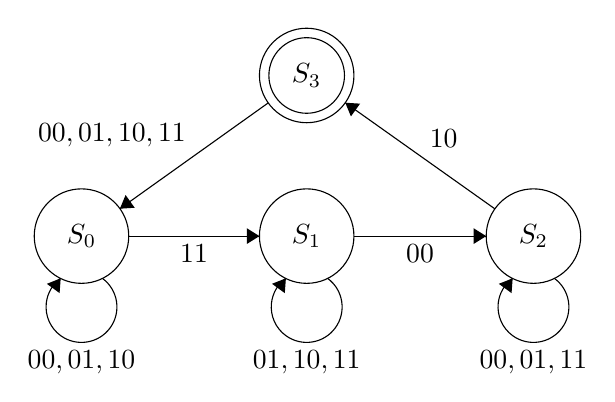
\begin{tikzpicture}[scale=0.2]
			\tikzstyle{every node}+=[inner sep=0pt]
			\draw [black] (17.4,-17.8) circle (3);
			\draw (17.4,-17.8) node {$S_0$};
			\draw [black] (31.7,-17.8) circle (3);
			\draw (31.7,-17.8) node {$S_1$};
			\draw [black] (46.1,-17.8) circle (3);
			\draw (46.1,-17.8) node {$S_2 $};
			\draw [black] (31.7,-7.6) circle (3);
			\draw (31.7,-7.6) node {$S_3$};
			\draw [black] (31.7,-7.6) circle (2.4);
			\draw [black] (20.4,-17.8) -- (28.7,-17.8);
			\fill [black] (28.7,-17.8) -- (27.9,-17.3) -- (27.9,-18.3);
			\draw (24.55,-18.3) node [below] {$11$};
			\draw [black] (34.7,-17.8) -- (43.1,-17.8);
			\fill [black] (43.1,-17.8) -- (42.3,-17.3) -- (42.3,-18.3);
			\draw (38.9,-18.3) node [below] {$00$};
			\draw [black] (43.65,-16.07) -- (34.15,-9.33);
			\fill [black] (34.15,-9.33) -- (34.51,-10.2) -- (35.09,-9.39);
			\draw (40.4,-12.2) node [above] {$10$};
			\draw [black] (18.723,-20.48) arc (54:-234:2.25);
			\draw (17.4,-25.05) node [below] {$00,01,10$};
			\fill [black] (16.08,-20.48) -- (15.2,-20.83) -- (16.01,-21.42);
			\draw [black] (33.023,-20.48) arc (54:-234:2.25);
			\draw (31.7,-25.05) node [below] {$01,10,11$};
			\fill [black] (30.38,-20.48) -- (29.5,-20.83) -- (30.31,-21.42);
			\draw [black] (47.423,-20.48) arc (54:-234:2.25);
			\draw (46.1,-25.05) node [below] {$00,01,11$};
			\fill [black] (44.78,-20.48) -- (43.9,-20.83) -- (44.71,-21.42);
			\draw [black] (29.26,-9.34) -- (19.84,-16.06);
			\fill [black] (19.84,-16.06) -- (20.78,-16) -- (20.2,-15.19);
			\draw (19.33,-12.2) node [above] {$00,01,10,11$};
		\end{tikzpicture}

		\end{figure}

		Hierbij is de output voor \(S_0, S_1\) en \(S_2\) gelijk aan \(Y=0\); de output voor \(S_3\) is gelijk aan \(Y=1\). Omdat de output enkel afhangt van de toestand, is dit inderdaad een Moore FSM.

		\item Toestandscodering:
		\begin{align*}
			\begin{array}{c c c}
				& \text{straight-forward} &\\
				S_0 & \rightarrow & 00 \\
				S_1 & \rightarrow & 01 \\
				S_2 & \rightarrow & 10 \\
				S_3 & \rightarrow & 11 \\
			\end{array} \qquad \qquad \begin{array}{c c c}
			& \text{Gray} &\\
			S_0 & \rightarrow & 00 \\
			S_1 & \rightarrow & 01 \\
			S_2 & \rightarrow & 11 \\
			S_3 & \rightarrow & 10 \\
			\end{array}
		\end{align*}
		Bij de straight-forward is de codering van een toestand simpelweg een binaire voorstelling van het aantal juiste cijfers die al werden ingegeven om in deze toestand te geraken. De naam zegt het zelf: de codering is straight-forward en makkelijk te begrijpen. De Gray codering zorgt voor een minimaal aantal bit-flips. Er verandert telkens 1 bit bij een overgang -- de overgangen \(S_0 \leftrightarrow S_2\) en \(S_1 \leftrightarrow S_3\) zijn immers onmogelijk.
	\end{enumerate}

\end{document}



